\lecture{5}{Oct 9 2024 Wed (13:02:05)}{Nested Interval Property}

\begin{theorem}[Nested Interval Property]
  For each $n \in \N$, assume we are given a closed interval $I_n = [a_n, b_n] = \left\{x \in \R \mid a_n \le x \le b_n\right\}$. Assume also that each $I_n$ contains the next interval, i.e., $I_n \supseteq I_{n+1}$. Then, the resulting sequence of closed intervals
  \[%
    I_1 \supseteq I_2 \supseteq I_3 \supseteq \cdots
  ,\]%
  has a nonempty intersection. That is,
  \[%
    \bigcap_{n=1}^\infty I_n \neq \emptyset
  .\]%
\end{theorem}

\begin{proof}
  Let $A = \{a_n : n \in \N\}$. Since $I_n \supseteq I_{n+1}$, we have $a_1 \le a_2 \le a_3 \le \cdots$ (the left endpoints are nondecreasing) and $b_1 \ge b_2 \ge b_3 \ge \cdots$ (the right endpoints are nonincreasing). Moreover, for each $n$ we have $a_n \le b_n \le b_1$, so $A$ is bounded above by $b_1$.

  By the Axiom of Completeness, $A$ has a least upper bound $s = \sup(A)$. Combining these inequalities, for every $n$ we have
  \[%
    a_n \le s \le b_n
  ,\]%
  which means $s \in I_n$ for all $n \in \N$. Hence
  \[%
    s \in \bigcap_{n=1}^\infty I_n
  ,\]%
  proving that the intersection is nonempty.
\end{proof}

The Nested Interval Property can be viewed graphically, as shown below.
\begin{figure}[H]
  \centering

  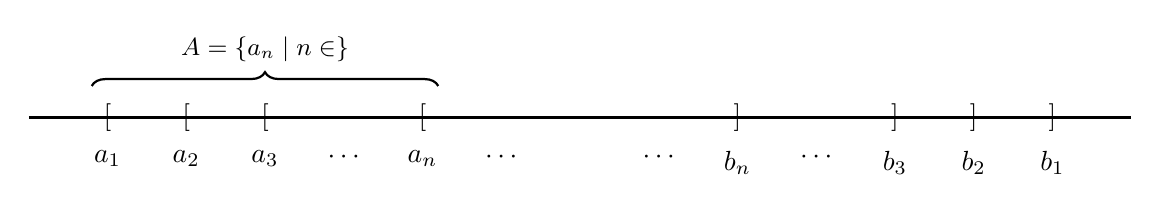
\begin{tikzpicture}
    \draw[thick] (-7, 0) -- (7, 0);

    \foreach \i/\pos in {1/-6, 2/-5, 3/-4, n/-2} {
      \node at (\pos, 0) {$[$};
      \node[below] at (\pos, -0.3) {$a_{\i}$};
    }
    \node[below] at (-3, -0.3) {$\cdots$};

    \foreach \i/\pos in {n/2, 3/4, 2/5, 1/6} {
      \node at (\pos, 0) {$]$};
      \node[below] at (\pos, -0.3) {$b_{\i}$};
    }
    \node[below] at (3, -0.3) {$\cdots$};

    \node[below] at (1, -0.3) {$\cdots$};
    \node[below] at (-1, -0.3) {$\cdots$};

    \draw[decorate,decoration={brace,amplitude=5pt},thick] (-6.2, 0.4) -- (-1.8, 0.4) node[midway, above=5pt] {{\small$A = \{a_n \mid n \in \N\}$}};
  \end{tikzpicture}
\end{figure}

\begin{example}\leavevmode
  \begin{enumerate}
    \item The interval $I_n = \left[0, \frac{1}{n}\right]$, which is clearly $I_n \supset I_{n+1}$, since $\bigcap_{n=1}^\infty = \{0\}$.

    \item The counter example is $I_n = \left(0, \frac{1}{n}\right)$, $\bigcap_{n=0}^\infty I_n = \emptyset$, since $0 \notin I_n$. \qedhere
  \end{enumerate}
\end{example}


\begin{proposition}
  The set $\N$ is unbounded.
\end{proposition}

\begin{proof}
  Assume, for contradiction, that $\N$ is bounded above. Then, it follows that we can set $\alpha = \sup(\N)$. If we consider $\alpha - 1$, then we no longer have an upper bound for $\N$, and therefore, there exists an $n \in \N$ satisfying $\alpha - 1 < n$, which is equivalent to $\alpha < n + 1$. Since we have $n + 1 \in \N$, this contradicts the assumption that $\alpha$ is the least upper bound of $\N$.
\end{proof}

\begin{theorem}[Archimedian Property]\leavevmode
  \begin{enumerate}
    \item $(\forall x \in \R)(\exists n \in \N)[n > x]$.

    \item $(\forall y > 0)(\exists n \in \N)[\sfrac{1}{n} < 1]$.
  \end{enumerate}
\end{theorem}

\begin{proof}\leavevmode
  \begin{enumerate}
    \item Property (i) follows given that $\N$ is unbounded.

    \item Apply property (i) with $x = \sfrac{1}{y} > 0$. \qedhere
  \end{enumerate}
\end{proof}
